\section{Stablecoin Opportunity Score}
\label{sec:sos}

\subsection{Construction}

We construct a Stablecoin Opportunity Score (SOS) that ranks countries by potential gains from alternative payment infrastructure. The SOS is built directly from the three panel coefficients estimated in Section~\ref{sec:results}: $\hat{\gamma}_{\text{FATF}} = -0.108$, $\hat{\gamma}_{\text{AMLD}} = +0.141$, $\hat{\gamma}_{\text{FDI}} = -0.135$.

For each country $c$, define the per-channel intensive score as the friction-elasticity-weighted sum of complex trade in the affected corridors:
\begin{align}
\text{SOS}^{\text{FATF}}_c &= |\hat{\gamma}_{\text{FATF}}| \sum_{j \in \mathcal{G}_c} \sum_{p: \text{RCA}_{cp} \geq 1} \text{PCI}_p \times \text{Trade}_{cjp,T}, \\
\text{SOS}^{\text{FDI}}_c  &= |\hat{\gamma}_{\text{FDI}}|  \sum_{j \in \mathcal{D}_c} \sum_{p: \text{RCA}_{cp} \geq 1} \text{PCI}_p \times \text{Trade}_{cjp,T}, \\
\text{SOS}^{\text{AMLD}}_c &= \hat{\gamma}_{\text{AMLD}}    \sum_{j \in \mathcal{E}_c} \sum_{p: \text{RCA}_{cp} \geq 1} \text{PCI}_p \times \text{Trade}_{cjp,T},
\end{align}
where $\mathcal{G}_c$ is the set of greylisted partners of $c$, $\mathcal{D}_c$ is the set of FDI-derisked partners, $\mathcal{E}_c$ is the set of EU partners (post-2017), $T = 2023$ is the latest sample year, and trade is summed over country $c$'s revealed-comparative-advantage products. The intensive-margin component is anchored on the $\hat{\gamma}$ coefficients estimated in Section~\ref{sec:results}; the extensive margin enters implicitly through the RCA filter in the inner sum, supported by the unconditional level effect of country-level de-risking on $\Pr(\text{RCA}\geq 1)$ but not by a complexity-specific differential at the country-product level. The level-effect estimate from Section~\ref{subsec:extensive} (Table~\ref{tab:extensive_panel}, $\hat{\beta}_{\text{PF}} = -0.50$, $p = 0.028$, on a friction share with sample range $[0,1]$) implies that a 10-percentage-point increase in the de-risked-partner share lowers the unconditional probability of RCA by roughly 5 percentage points. The composite is therefore best read as a policy index that aggregates the strongly identified intensive-margin effects with a weakly identified extensive-margin level effect.

The composite SOS aggregates the two negative-shock channels and subtracts the AMLD term:
\begin{equation}
\text{SOS}^{\text{composite}}_c = \widetilde{\text{SOS}}^{\text{FATF}}_c + \widetilde{\text{SOS}}^{\text{FDI}}_c - \widetilde{\text{SOS}}^{\text{AMLD}}_c,
\label{eq:sos_composite}
\end{equation}
where tildes denote min-max normalization to a 0--10 scale within each channel. The minus sign on the AMLD term encodes the substitution argument from Section~\ref{sec:results}: countries already covered by EU regulatory harmonization need stablecoins less, because AMLD harmonization is a partial substitute for an alternative settlement layer.

\subsection{The composite is a weighted-evidence aggregator, not a robustness check}
\label{subsec:sos_framing}

The two single-instrument rankings, $\text{SOS}^{\text{FATF}}_c$ and $\text{SOS}^{\text{FDI}}_c$, are themselves weakly correlated. Spearman rank correlations are $\rho(\text{FDI}, \text{FATF}) = 0.249$, $\rho(\text{FDI}, \text{composite}) = 0.487$, and $\rho(\text{FATF}, \text{composite}) = 0.429$ (Table~\ref{tab:sos_corr}). The two single-instrument rankings identify substantively different sets of exposed countries: FATF picks out greylisted economies (Croatia, Turkey, Bulgaria, Jordan, Barbados), while FDI picks out persistently de-risked economies (Fiji, Haiti, Nicaragua, Madagascar, Lebanon).

\begin{table}[htbp]
\centering
\caption{Spearman Rank Correlations Across SOS Variants}
\label{tab:sos_corr}
\begin{threeparttable}
\small
\begin{tabular}{lccc}
\toprule
 & SOS$_{\text{FDI}}$ & SOS$_{\text{FATF}}$ & SOS$_{\text{composite}}$ \\
\midrule
SOS FDI & 1.000 & 0.249 & 0.487 \\
SOS FATF & 0.249 & 1.000 & 0.429 \\
SOS composite & 0.487 & 0.429 & 1.000 \\
\bottomrule
\end{tabular}
\begin{tablenotes}
\tablenote{Spearman rank correlations across $N = 226$ countries. SOS$_{\text{FDI}}$ uses only the FDI-derisked channel; SOS$_{\text{FATF}}$ uses only the FATF greylist channel; SOS$_{\text{composite}}$ aggregates both negative-shock channels and subtracts the AMLD term as in equation~(\ref{eq:sos_composite}).}
\end{tablenotes}
\end{threeparttable}
\end{table}

The composite is therefore not a robustness check on the rank order across $\gamma$ choices. It is a weighted-evidence aggregator across two distinct identification strategies that measure overlapping but non-identical exposure. We defend it on conceptual grounds: each negative-shock channel is a valid causal estimate, and aggregating both channels integrates evidence across two natural experiments rather than choosing one. Of the 226 countries, 152 shift quintile from the FDI-only ranking to the composite, and 155 shift quintile from the FATF-only ranking. The composite necessarily re-orders the rankings by design.

Figure~\ref{fig:ranking_corr} visualizes the pairwise rank correlations across the three SOS variants. The scatter plots show the moderate correspondence between FDI- and FATF-only rankings ($\rho = 0.249$) and the stronger correspondence each has with the composite ($\rho = 0.487$ and $\rho = 0.429$).

\begin{figure}[htbp]
\centering
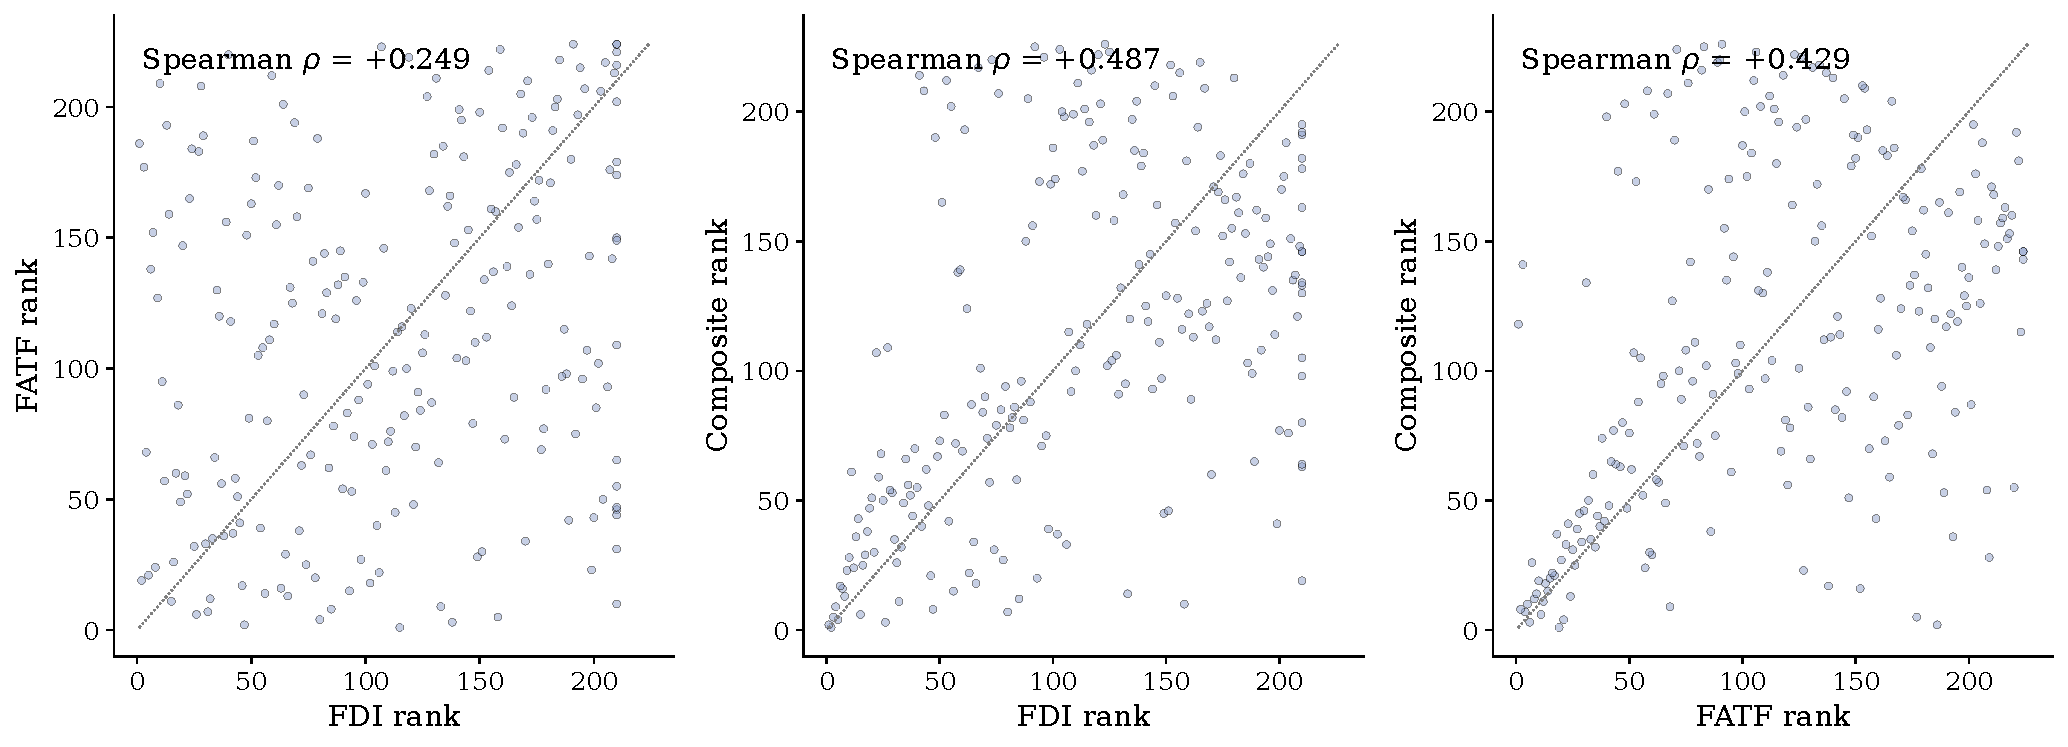
\includegraphics[width=0.85\textwidth]{figures/13_figures/fig_ranking_correlations.pdf}
\caption{Pairwise Rank Correlations Across SOS Variants}
\label{fig:ranking_corr}
\begin{minipage}{0.9\textwidth}
\footnotesize \textit{Notes.} Pairwise scatter plots of country ranks under the FDI-only, FATF-only, and composite SOS variants. Spearman correlations: $\rho(\text{FDI},\text{FATF}) = 0.249$, $\rho(\text{FDI},\text{composite}) = 0.487$, $\rho(\text{FATF},\text{composite}) = 0.429$. $N = 226$ countries.
\end{minipage}
\end{figure}

The negative AMLD adjustment encodes a separate substantive claim: regulatory clarity is a partial substitute for stablecoin payment rails. EU members appear lower in the composite ranking than they would in a single-instrument ranking that ignores AMLD harmonization. This down-weighting is the policy point. Stablecoins are a substitute for missing harmonization, not an across-the-board upgrade.

\subsection{Country rankings}

Table~\ref{tab:sos_top20} presents the top 20 countries by composite SOS. Haiti ranks first (10.8), driven by a high FDI-de-risked footprint (5 derisked partners, large complex-trade exposure) combined with greylisting in part of the sample. Fiji ranks second (9.3) on FDI exposure alone (12 de-risked partners, near-zero greylisting). Syria (8.1) and Lebanon (7.4) combine high greylisting and de-risking exposure with limited regulatory harmonization. Nicaragua (7.3) rounds out the top five.

\begin{table}[htbp]
\centering
\caption{Top 20 Countries by Composite Stablecoin Opportunity Score}
\label{tab:sos_top20}
\begin{threeparttable}
\scriptsize
\begin{tabular}{clcccccccc}
\toprule
Rank & Country & Composite & FATF & FDI & AMLD & De-risked & Trade at risk & Rank low & Rank high \\
 & & SOS & SOS & SOS & adj. & partners & (USD M) & ($\gamma$ low) & ($\gamma$ high) \\
\midrule
1 & HTI & 10.83 & 3.30 & 7.64 & 0.12 & 5 & 0.9 & 1 & 1 \\
2 & FJI & 9.26 & 0.06 & 9.60 & 0.40 & 12 & 0.6 & 87 & 4 \\
3 & SYR & 8.10 & 6.67 & 2.11 & 0.68 & 13 & 0.1 & 38 & 5 \\
4 & LBN & 7.36 & 3.09 & 5.46 & 1.19 & 24 & 1.3 & 154 & 8 \\
5 & NIC & 7.31 & 0.08 & 7.44 & 0.21 & 5 & 4.8 & 48 & 14 \\
6 & SEN & 7.28 & 5.10 & 2.67 & 0.49 & 18 & 1.1 & 19 & 10 \\
7 & JOR & 7.25 & 6.90 & 0.73 & 0.38 & 11 & 0.6 & 2 & 9 \\
8 & TUR & 6.74 & 8.30 & 1.22 & 2.79 & 23 & 13.9 & 186 & 3 \\
9 & MDG & 6.69 & 0.66 & 7.29 & 1.27 & 19 & 2.2 & 165 & 11 \\
10 & BRB & 6.49 & 6.88 & 0.20 & 0.59 & 10 & 0.0 & 13 & 12 \\
11 & TZA & 6.43 & 4.96 & 1.84 & 0.37 & 37 & 1.6 & 7 & 15 \\
12 & VNM & 6.22 & 6.27 & 0.65 & 0.71 & 7 & 14.7 & 56 & 13 \\
13 & NGA & 6.15 & 2.47 & 4.58 & 0.90 & 71 & 39.3 & 135 & 16 \\
14 & UGA & 5.44 & 5.70 & 0.31 & 0.56 & 17 & 0.1 & 37 & 17 \\
15 & PHL & 5.07 & 4.31 & 1.09 & 0.33 & 48 & 8.5 & 10 & 19 \\
16 & AFG & 4.89 & 0.20 & 4.76 & 0.07 & 8 & 0.7 & 20 & 26 \\
17 & GRD & 4.87 & 0.25 & 5.29 & 0.68 & 4 & 0.0 & 129 & 21 \\
18 & JAM & 4.78 & 4.33 & 0.92 & 0.47 & 8 & 0.1 & 42 & 20 \\
19 & ZAF & 4.71 & 5.30 & 0.00 & 0.59 & 0 & 0.0 & 51 & 18 \\
20 & YEM & 4.66 & 4.23 & 0.56 & 0.14 & 7 & 0.1 & 3 & 24 \\
\bottomrule
\end{tabular}
\begin{tablenotes}
\tablenote{SOS$_{\text{composite}}$ aggregates FATF and FDI single-instrument scores and subtracts the AMLD adjustment as in equation~(\ref{eq:sos_composite}). ``FATF SOS,'' ``FDI SOS,'' and ``AMLD adj.'' report the channel components on the same 0--10 normalized scale. ``De-risked partners'' counts country $c$'s partners with FDI ratio below 0.5. ``Trade at risk (USD M)'' is the dollar-weighted intensive-margin exposure across all three channels for 2023. Rank low and Rank high report the country's rank under the composite using $\hat{\gamma}_{\text{low}}$ and $\hat{\gamma}_{\text{high}}$ at the channel-specific 95\% confidence-interval bounds.}
\end{tablenotes}
\end{threeparttable}
\end{table}

The composite ranking concentrates among small economies with high greylisting and de-risking exposure. Of the top 20, 14 are classified by the World Bank as low- or lower-middle-income, and 17 have populations under 25 million. The presence of Turkey (rank~8), Vietnam (rank~12), and Nigeria (rank~13) reflects large absolute trade volumes through high-friction corridors rather than per-corridor exposure. Larger advanced economies, which dominate the FDI-only ranking when the AMLD adjustment is omitted, fall in the composite because their EU partners receive negative AMLD weight.

Figure~\ref{fig:sos_decomp_main} decomposes the composite into its FATF, FDI, and AMLD components for the top-20 countries.

\begin{figure}[htbp]
\centering
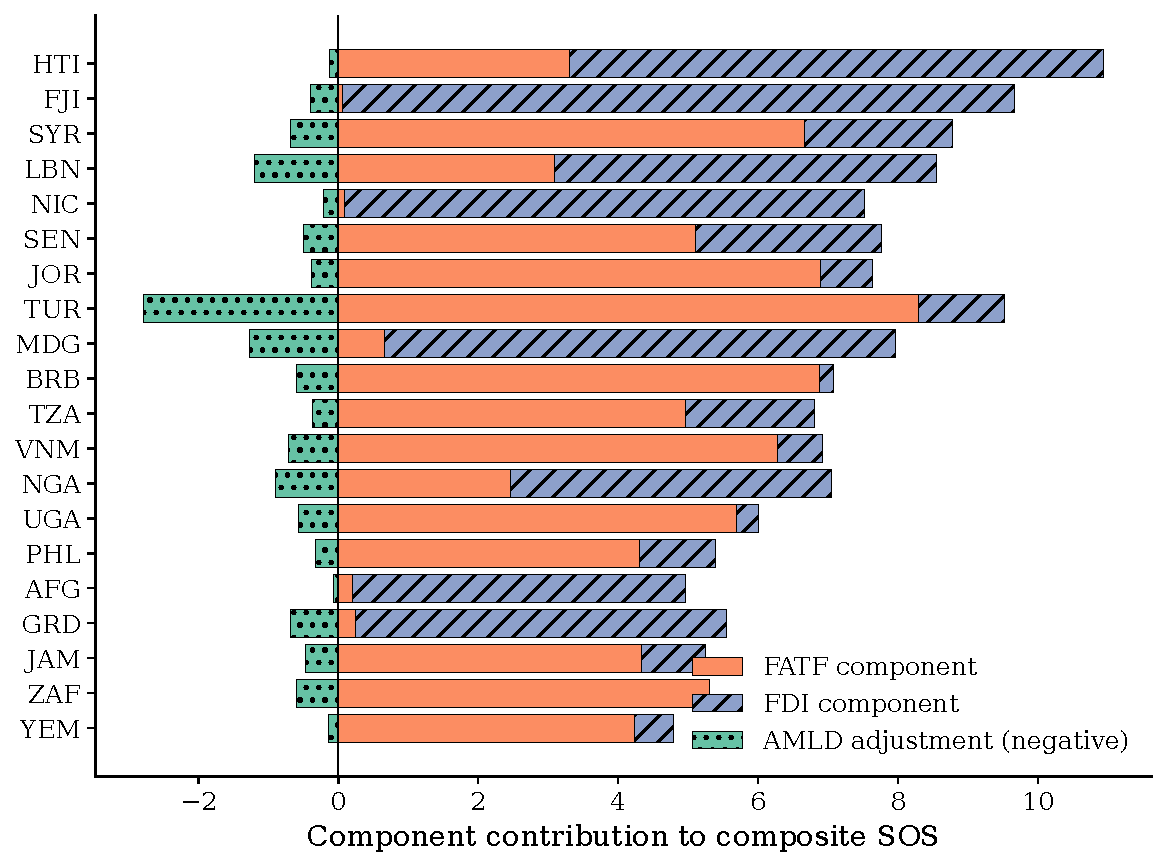
\includegraphics[width=0.8\textwidth]{figures/13_figures/fig_sos_decomposition.pdf}
\caption{Composite SOS: FATF, FDI, and AMLD Components}
\label{fig:sos_decomp_main}
\begin{minipage}{0.9\textwidth}
\footnotesize \textit{Notes.} Stacked decomposition of the top-20 composite SOS into its FATF, FDI, and AMLD components. The AMLD component enters with a negative sign per equation~(\ref{eq:sos_composite}). Components are on the 0--10 normalized scale.
\end{minipage}
\end{figure}

Figure~\ref{fig:world_sos} maps the composite SOS globally. High-opportunity countries cluster in the Caribbean, Sub-Saharan Africa, the Levant, South and Southeast Asia, and the Pacific.

\begin{figure}[htbp]
\centering
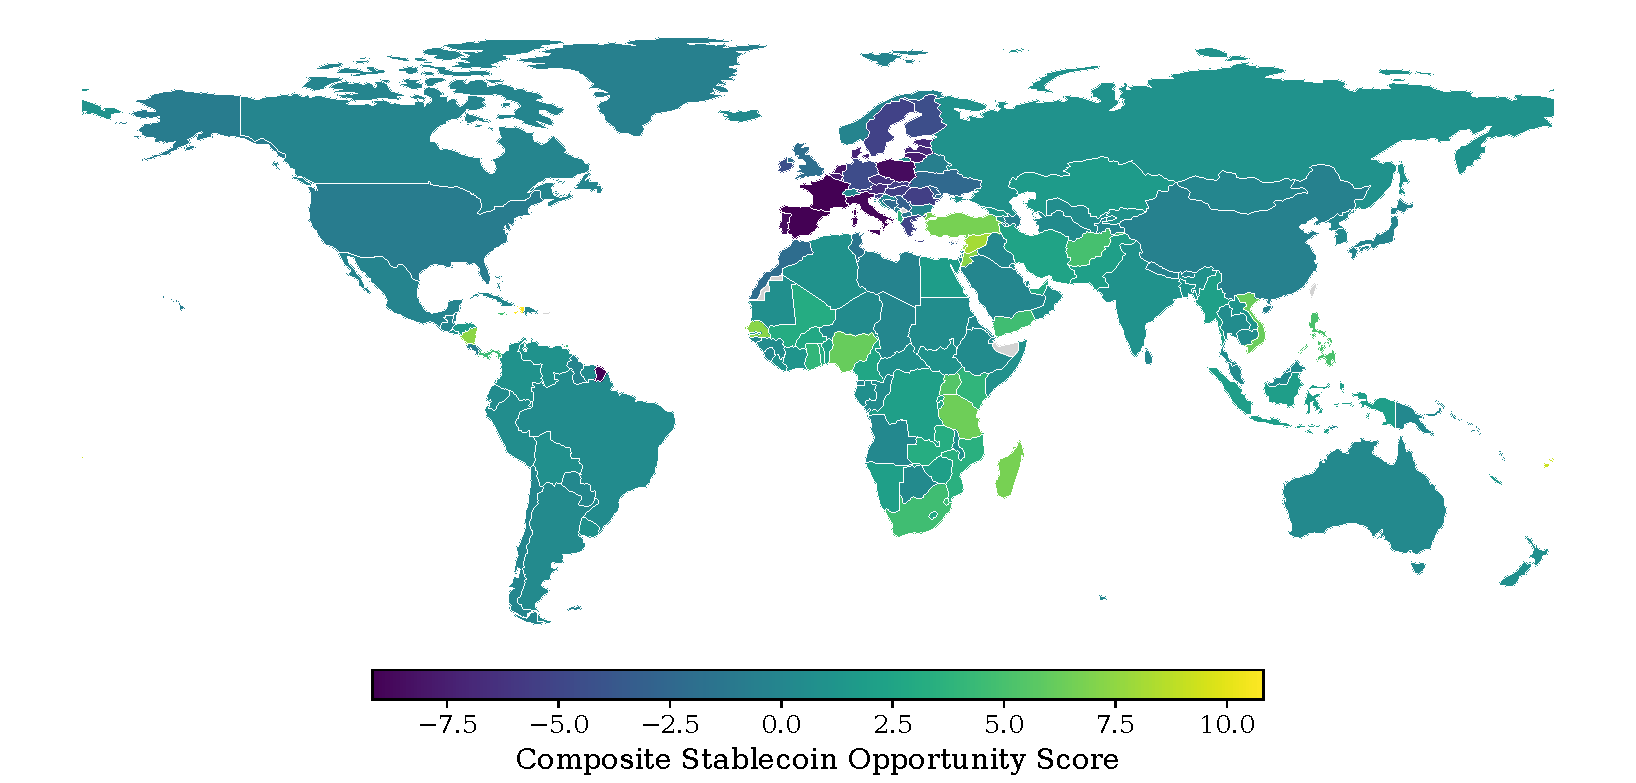
\includegraphics[width=0.95\textwidth]{figures/13_figures/world_heatmap_sos.pdf}
\caption{Composite Stablecoin Opportunity Score: World Map}
\label{fig:world_sos}
\begin{minipage}{0.9\textwidth}
\footnotesize \textit{Notes.} Country-level composite Stablecoin Opportunity Score, plotted as a choropleth using Natural Earth low-resolution country polygons. Brighter shading indicates higher composite SOS; countries with no data shown in light gray. The composite incorporates the AMLD adjustment, so EU members appear lower than they would in a single-instrument ranking.
\end{minipage}
\end{figure}

Figure~\ref{fig:sos_gdppc} plots SOS against GDP per capita. The composite SOS is not simply a proxy for income level: high-SOS countries span the income distribution, with large absolute trade exposure in middle-income economies (Turkey, Vietnam, Nigeria) and high per-corridor exposure in low-income economies (Haiti, Madagascar, Yemen).

\begin{figure}[htbp]
\centering
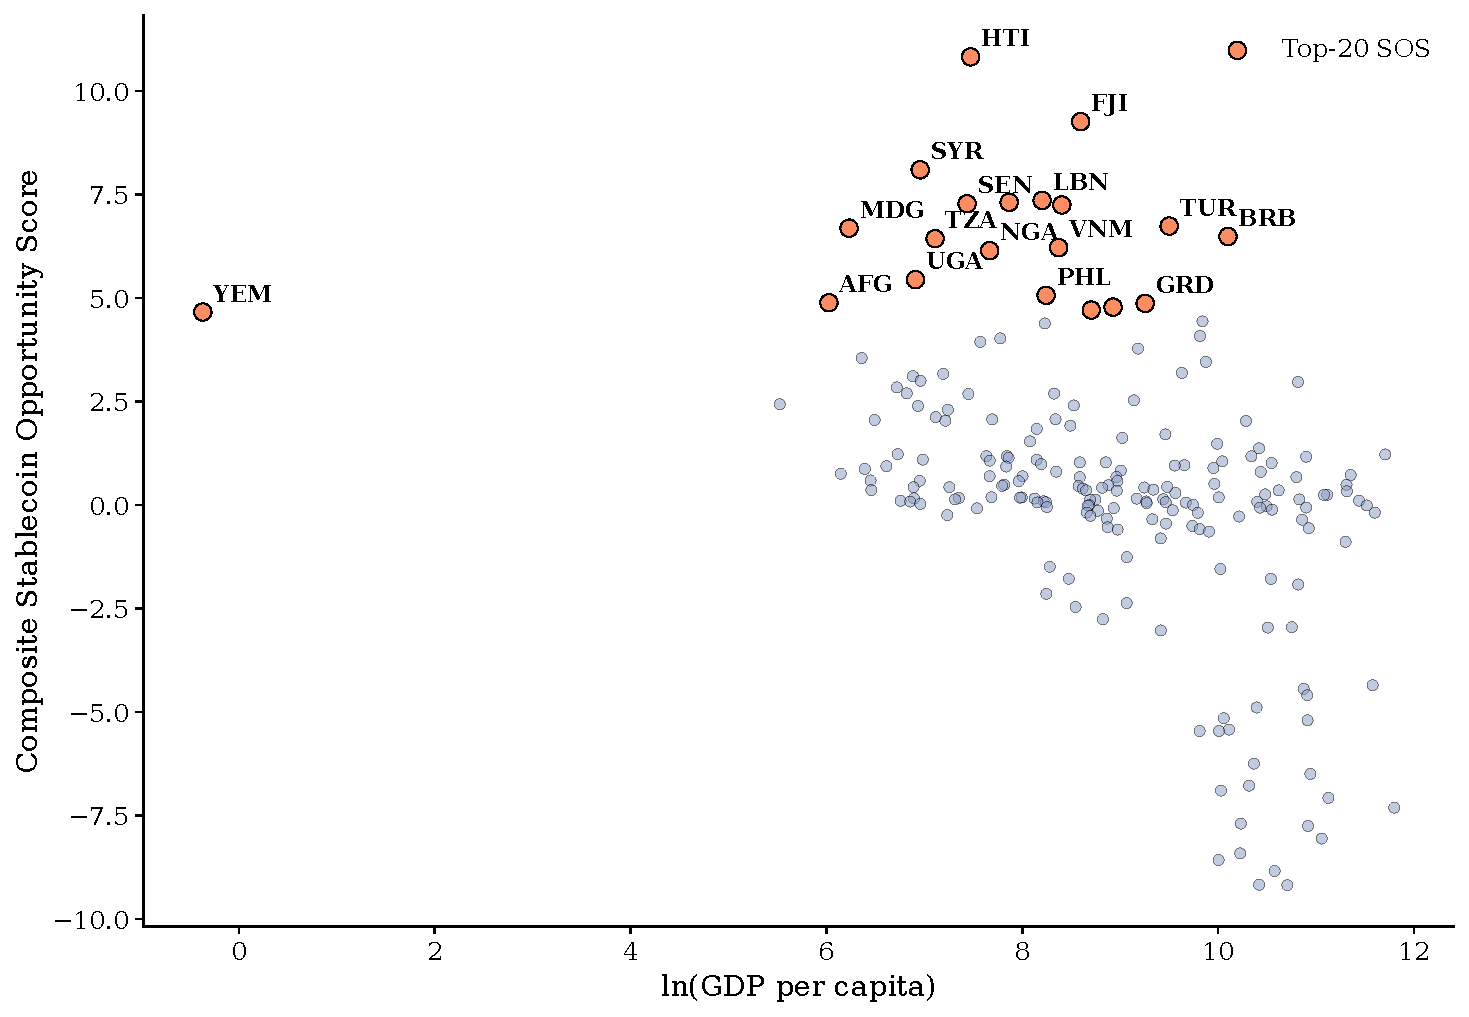
\includegraphics[width=0.7\textwidth]{figures/13_figures/sos_vs_gdppc.pdf}
\caption{Composite SOS versus GDP per Capita}
\label{fig:sos_gdppc}
\begin{minipage}{0.9\textwidth}
\footnotesize \textit{Notes.} Each point is a country. Horizontal axis: log GDP per capita. Labels shown for top 10 composite SOS countries.
\end{minipage}
\end{figure}

\subsection{Feasibility quadrant}
\label{subsec:quadrant}

High-SOS countries differ in their ability to deploy stablecoins immediately. We classify countries along two dimensions: (i) capital-account openness, measured by the Chinn-Ito KAOPEN index, and (ii) infrastructure readiness, proxied by log GDP per capita. The GDP-per-capita proxy is a placeholder: Chainalysis's Global Crypto Adoption Index, the preferred infrastructure measure, is deferred to a future revision. Thresholds are set at the median of each axis. Table~\ref{tab:quadrant} reports the resulting four quadrants.

\begin{table}[htbp]
\centering
\caption{Feasibility Quadrant Summary}
\label{tab:quadrant}
\begin{threeparttable}
\small
\begin{tabular}{lccl}
\toprule
Quadrant & N & Mean SOS & Top-3 (by SOS) \\
\midrule
Q1: Actionable now & 60 & -2.181 & PAN, TTO, ARE \\
Q2: Infrastructure gap & 23 & 2.519 & HTI, LBN, NIC \\
Q3: Legal complexity (sandbox) & 15 & 1.773 & TUR, BRB, GRD \\
Q4: Structurally blocked & 63 & 1.764 & FJI, SYR, SEN \\
\bottomrule
\end{tabular}

\begin{tablenotes}
\tablenote{Q1 (Actionable now): open capital account and above-median infrastructure readiness. Q2 (Infrastructure gap): open capital account, below-median infrastructure. Q3 (Legal complexity, sandbox): above-median infrastructure, restricted capital account. Q4 (Structurally blocked): below-median infrastructure and restricted capital account. Thresholds set at the median of KAOPEN and log GDP per capita. Infrastructure readiness uses log GDP per capita as a placeholder; the Chainalysis Global Crypto Adoption Index is deferred to a future revision. 65 countries are unclassified due to missing KAOPEN or GDP-per-capita data.}
\end{tablenotes}
\end{threeparttable}
\end{table}

The four quadrants partition the 161 classified countries unevenly. Q1 (actionable now) contains 60 countries with both an open capital account and above-median infrastructure. Q1's mean composite SOS is $-2.18$, the lowest of the four quadrants, because high-SOS countries select into Q2 and Q4 by construction: SOS targets corridors with high friction exposure (greylisting, FDI de-risking), which correlates with restricted capital accounts or below-median infrastructure. The actionable signal in Q1 therefore lies in the within-quadrant ranking, not the quadrant mean. Q2 (infrastructure gap) contains 23 countries that have an open capital account but lack infrastructure; this quadrant holds the highest mean composite SOS at $+2.52$, indicating that the largest unmet opportunity sits in capital-open economies where infrastructure has not yet caught up. Q3 (legal complexity, sandbox) contains 15 countries where infrastructure exists but capital-account restrictions force a regulatory-sandbox approach. Q4 (structurally blocked) contains 63 countries that face both barriers; this is the largest quadrant by count and the hardest deployment environment.

The composition of the actionable quadrant is informative. Table~\ref{tab:actionable_top10} lists the top 10 Q1 countries by composite SOS: Panama, Trinidad and Tobago, the United Arab Emirates, Bahrain, Georgia, San Marino, Uruguay, Oman, Armenia, and Kuwait. The list concentrates among small open economies and Gulf financial centers. These are jurisdictions where capital flows freely and basic financial infrastructure is in place, so a stablecoin-rail rollout faces neither a capital-controls bottleneck nor a primary-infrastructure shortage.

\begin{table}[htbp]
\centering
\caption{Q1 (Actionable Now): Top 10 Countries by Composite SOS}
\label{tab:actionable_top10}
\begin{threeparttable}
\small
\begin{tabular}{lcccc}
\toprule
ISO3 & SOS composite & Rank (overall) & KAOPEN & ln(GDPpc) \\
\midrule
PAN & 4.436 & 21 & 1.000 & 9.841 \\
TTO & 4.084 & 23 & 0.659 & 9.815 \\
ARE & 2.974 & 33 & 1.000 & 10.817 \\
BHR & 2.031 & 48 & 1.000 & 10.285 \\
GEO & 1.624 & 52 & 1.000 & 9.022 \\
SMR & 1.169 & 61 & 0.702 & 10.900 \\
URY & 1.056 & 66 & 1.000 & 10.044 \\
OMN & 0.893 & 75 & 0.821 & 9.954 \\
ARM & 0.833 & 77 & 1.000 & 9.007 \\
KWT & 0.800 & 79 & 0.702 & 10.436 \\
\bottomrule
\end{tabular}

\begin{tablenotes}
\tablenote{Top 10 countries in Q1 (actionable now) ranked by composite SOS. ``Rank (overall)'' is the country's position in the full 226-country composite ranking from Table~\ref{tab:sos_top20}. KAOPEN is the Chinn-Ito capital-account openness index, normalized to $[0,1]$. ln(GDPpc) is log GDP per capita in 2023.}
\end{tablenotes}
\end{threeparttable}
\end{table}

Figure~\ref{fig:quadrant} maps the classification.

\begin{figure}[htbp]
\centering
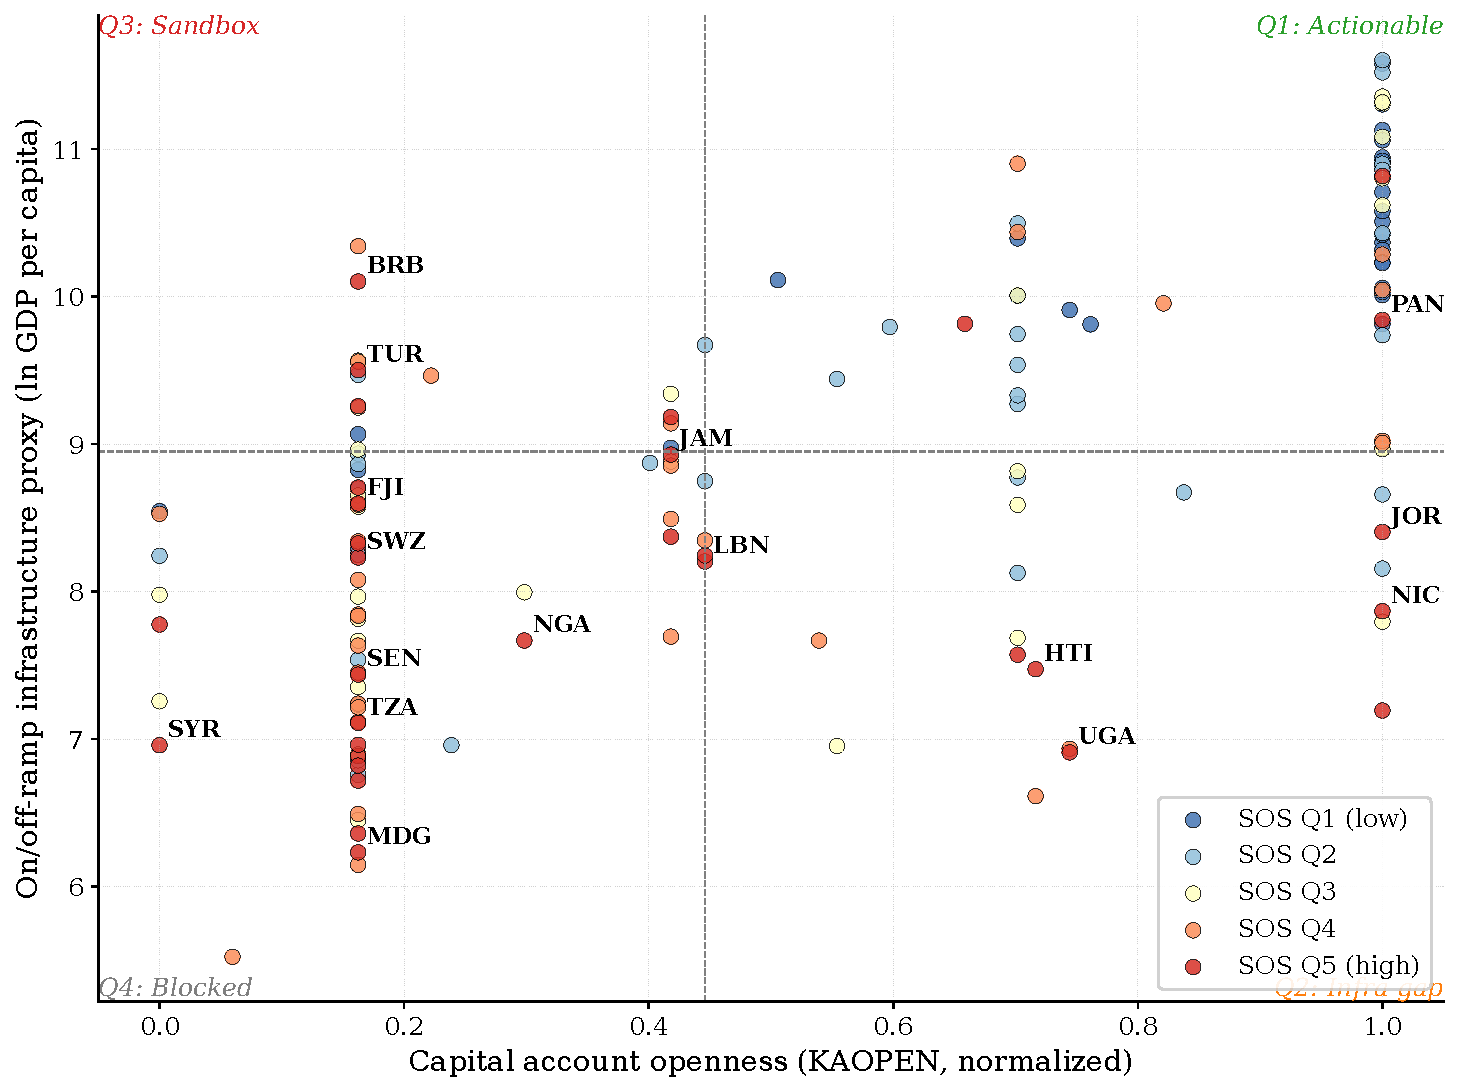
\includegraphics[width=0.8\textwidth]{figures/14_feasibility_quadrant/quadrant_scatter.pdf}
\caption{Feasibility Quadrant: Capital Openness vs.\ Infrastructure Readiness}
\label{fig:quadrant}
\begin{minipage}{0.9\textwidth}
\footnotesize \textit{Notes.} Each point is a country, sized by composite SOS. Horizontal axis: KAOPEN (capital-account openness). Vertical axis: log GDP per capita as an infrastructure-readiness placeholder. Dashed lines indicate median thresholds. Q1 (top right): actionable now. Q2 (bottom right): infrastructure gap. Q3 (top left): legal complexity. Q4 (bottom left): structurally blocked.
\end{minipage}
\end{figure}

Combining the SOS ranking with the feasibility quadrant produces a sharper policy reading than either dimension alone. Many of the top-ranked composite-SOS countries (Haiti, Fiji, Syria, Lebanon, Nicaragua) sit in Q2 or Q4, where deployment requires infrastructure investment or works around capital-account restrictions. The actionable quadrant is dominated by mid-sized open economies and small financial hubs whose absolute SOS is moderate but whose deployment friction is low.

\subsection{External validation}

We validate the composite SOS against the Chainalysis Global Crypto Adoption Index, which measures actual cryptocurrency usage across 149 countries. The unconditional Spearman rank correlation is $\rho = 0.155$; conditional on log GDP per capita, $\rho = 0.126$. The weak positive correlation is expected: composite SOS measures structural opportunity (unmet need for payment infrastructure), while Chainalysis measures current adoption. High-SOS countries are beginning to adopt (positive correlation), but many high-opportunity countries have not yet adopted crypto at scale (weak correlation). The two measures capture distinct constructs, and the composite SOS adds information beyond what current adoption data provide.
